\documentclass[11pt,a4paper]{article}

\usepackage[utf8]{inputenc}
\usepackage[T1]{fontenc}
\usepackage[margin=2.5cm]{geometry}
\usepackage{booktabs}
\usepackage{array}
\usepackage{graphicx}
\usepackage{amsmath}
\usepackage{float}
\usepackage{caption}
\usepackage[hidelinks]{hyperref}
\usepackage{xcolor}
\usepackage{listings}
\usepackage{tikz}
\usetikzlibrary{positioning,arrows.meta}

\lstset{
  language=Python,
  basicstyle=\ttfamily\small,
  keywordstyle=\color{blue!60!black},
  commentstyle=\color{gray},
  frame=single,
  columns=fullflexible,
  keepspaces=true,
}

\graphicspath{{figures/}}

% Every number quoted in running text comes from here, so prose and tables
% cannot disagree.  Regenerate with scripts/make_report_assets.py.
% Generated by scripts/make_report_assets.py -- do not edit.
% Re-run the script instead; every number here comes from results/.

\newcommand{\BestModel}{distilbert}
\newcommand{\BestAUC}{0.9898}
\newcommand{\BestAUCStd}{0.0011}
\newcommand{\BestPRAUC}{0.7193}
\newcommand{\BestMacroF}{0.6827}
\newcommand{\RunnerUpModel}{logreg}
\newcommand{\RunnerUpAUC}{0.9841}
\newcommand{\FoldStrategy}{iterative}
\newcommand{\NFolds}{5}
\newcommand{\NComments}{159{,}571}
\newcommand{\NModels}{6}
\newcommand{\RandomSeed}{42}
\newcommand{\PythonVersion}{3.14.0}
\newcommand{\SklearnVersion}{1.9.1}
\newcommand{\RunTimestamp}{2026-10-26T06:35:54+00:00}


\title{Toxic Comment Classification\\[0.3em]
  \large Seminar project, topic 3: multi-label classification of the Jigsaw corpus}
\author{Group members: \textit{(names and student IDs)}\\[0.3em]
  \small Course teacher: Assoc.\ Prof.\ Phuong T.\ Nguyen, University of L'Aquila}
\date{\today}

\begin{document}
\maketitle

\begin{abstract}
We study the Jigsaw Toxic Comment Classification Challenge, a multi-label task
in which each of \NComments{} Wikipedia talk-page comments may carry any subset
of six labels: \emph{toxic}, \emph{severe\_toxic}, \emph{obscene},
\emph{threat}, \emph{insult} and \emph{identity\_hate}.  We compare two trivial
baselines, three linear classifiers over word and character TF-IDF features and
a fine-tuned DistilBERT under \NFolds-fold multi-label stratified cross
validation, with per-label decision thresholds tuned inside each training fold.
The best model, \BestModel, reaches a mean column-wise ROC-AUC of
\BestAUC{}~$\pm$~\BestAUCStd, ahead of the best linear model, \RunnerUpModel{}
(\RunnerUpAUC), and far ahead of a profanity-list baseline (0.78).  The
aggregate hides two weaknesses: the rarest labels remain hard (PR-AUC between
0.50 and 0.61 for \emph{severe\_toxic}, \emph{threat} and
\emph{identity\_hate}), and both model families are biased against identity
terms -- a clean comment mentioning \emph{gay} is flagged as toxic 6.8 times as
often as the average clean comment by DistilBERT, and 10.5 times by logistic
regression.
\end{abstract}

\tableofcontents
\newpage

% =========================================================================== %
\section{Introduction}
% =========================================================================== %

Online platforms rely on automatic moderation to keep discussions civil, and
the first step of any such system is a classifier that recognises abusive
language.  The Jigsaw Toxic Comment Classification Challenge, hosted on Kaggle
by Jigsaw and Google in 2018, frames this as a \emph{multi-label} problem: a
comment is not merely toxic or clean, it can be at once obscene, insulting and
hateful towards an identity group.

The project brief asks us to implement machine learning or deep learning
classifiers, evaluate them with suitable metrics under $k$-fold cross
validation, compare them with dedicated baselines, and analyse the results.
We organise the study around four research questions:

\begin{description}
  \item[RQ1] Which model classifies toxic comments best, and is its gain over
        simple baselines worth the cost?
  \item[RQ2] How do the models cope with rare labels and label imbalance?
  \item[RQ3] How reliable are the cross-validated results?
  \item[RQ4] What errors remain, and are the models biased against identity
        groups?
\end{description}

Our contributions are:

\begin{itemize}
  \item a reproducible pipeline in Python that cross-validates every model on
        one shared fold assignment, so that models can be compared pairwise;
  \item a comparison of six models, from a constant predictor to a fine-tuned
        transformer, with the competition's metric and with metrics that
        expose the rare labels, and a check of the linear models on the
        official test set;
  \item an analysis of what the best model gets wrong: an error taxonomy built
        from concrete examples, violations of the label hierarchy, and an audit
        of unintended bias against identity terms.
\end{itemize}

% =========================================================================== %
\section{Related work}
% =========================================================================== %

\paragraph{The data.}  The corpus comes from the Wikipedia Detox project of
Wulczyn et al.~\cite{wulczyn2017}, who crowd-sourced annotations of talk-page
comments and found that a classifier could perform comparably to the
aggregated judgement of several annotators.  Jigsaw and Google released an extended version as the Toxic
Comment Classification Challenge~\cite{jigsaw2018}, with the six labels used
here.

\paragraph{Models.}  Linear models over n-gram features are strong baselines
for short-text classification; NB-SVM~\cite{wang2012} improves them by
rescaling the features with Naive Bayes log-count ratios and was a widely
used baseline in the competition.  Many of the top competition entries
ensembled recurrent neural networks over pre-trained word embeddings.  Pre-trained
transformers such as BERT~\cite{devlin2019} have since become the standard
approach to text classification; DistilBERT~\cite{sanh2019} compresses BERT
by knowledge distillation at a small cost in accuracy, which makes
fine-tuning feasible on a laptop GPU.

\paragraph{Unintended bias.}  Dixon et al.~\cite{dixon2018} showed on this
same data that toxicity classifiers learn to associate identity terms such as
\emph{gay} with toxicity, and measured it by comparing error rates on
synthetic sentences that mention different identities.  Borkan et
al.~\cite{borkan2019} proposed threshold-free subgroup metrics, which became
the evaluation of Jigsaw's follow-up competition on unintended bias.  Our
audit (Section~\ref{sec:bias}) follows the same idea -- comparing the
false-positive rate on comments that mention a term with the background rate
-- on real comments rather than synthetic ones.

% =========================================================================== %
\section{Dataset}
% =========================================================================== %

The training set contains \NComments{} comments, each with six binary labels.
As the brief requires, models are compared by $k$-fold cross validation on the
training set.  The competition's test set was labelled only after the
competition closed, and only partially (63,978 of 153,164 rows are usable); we
use those rows once, at the end, to check how the cross-validated numbers
transfer to unseen data (Section~\ref{sec:testset}).

\subsection{Label frequency}

The labels are rare and severely imbalanced (Figure~\ref{fig:freq}): 89.8\% of
the comments carry no label at all, \emph{toxic} occurs in 9.6\% of the
comments, and \emph{threat} in only 0.3\% -- 478 comments in the whole corpus,
about 96 per validation fold.  Accuracy is therefore meaningless: the
constant ``clean'' prediction is right on nine comments out of ten.

\begin{figure}[H]
  \centering
  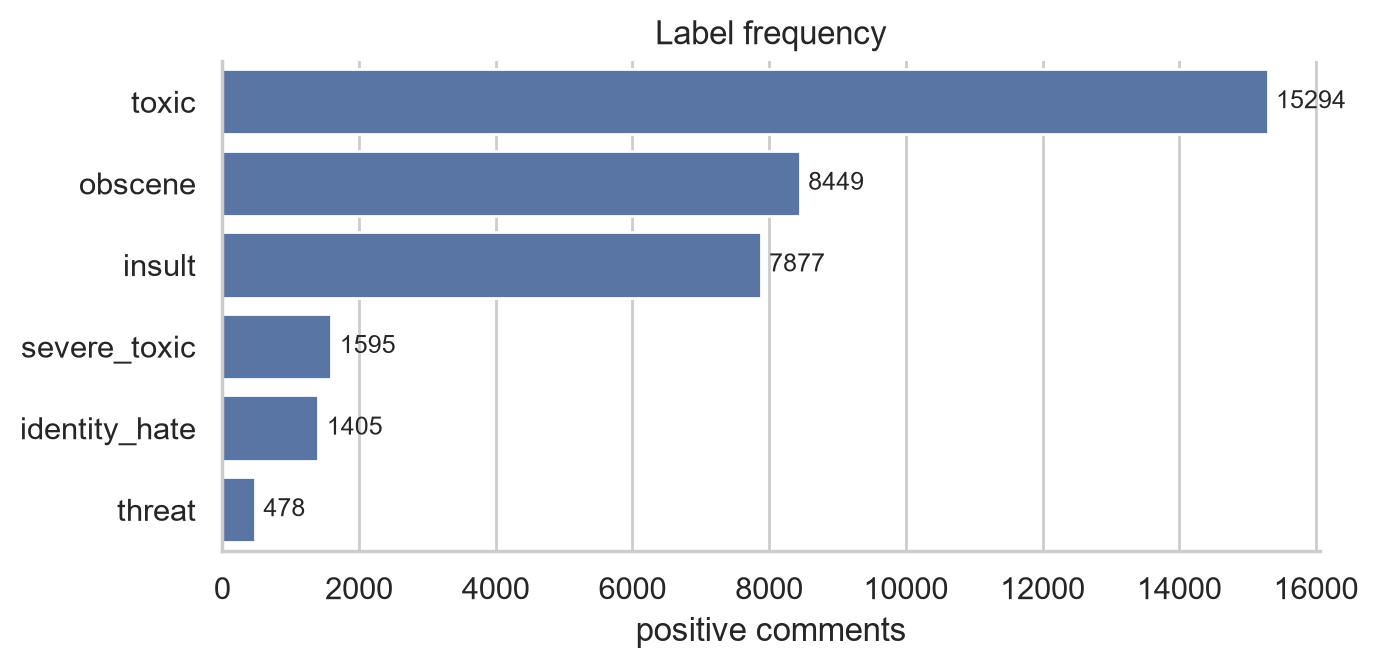
\includegraphics[width=0.75\linewidth]{label_frequency}
  \caption{Number of positive comments per label.}
  \label{fig:freq}
\end{figure}

\subsection{Label co-occurrence and hierarchy}

The labels are strongly correlated (Figure~\ref{fig:cooc}).  \emph{severe\_toxic}
is a strict subset of \emph{toxic}: $P(\text{toxic} \mid \text{severe\_toxic}) =
1$.  The other four labels co-occur with \emph{toxic} in 93--94\% of cases but
not always (for instance 523 obscene comments are not labelled toxic).  A
binary-relevance model, which trains each label independently, ignores this
structure; Section~\ref{sec:hierarchy} measures what that costs.

\begin{figure}[htbp]
  \centering
  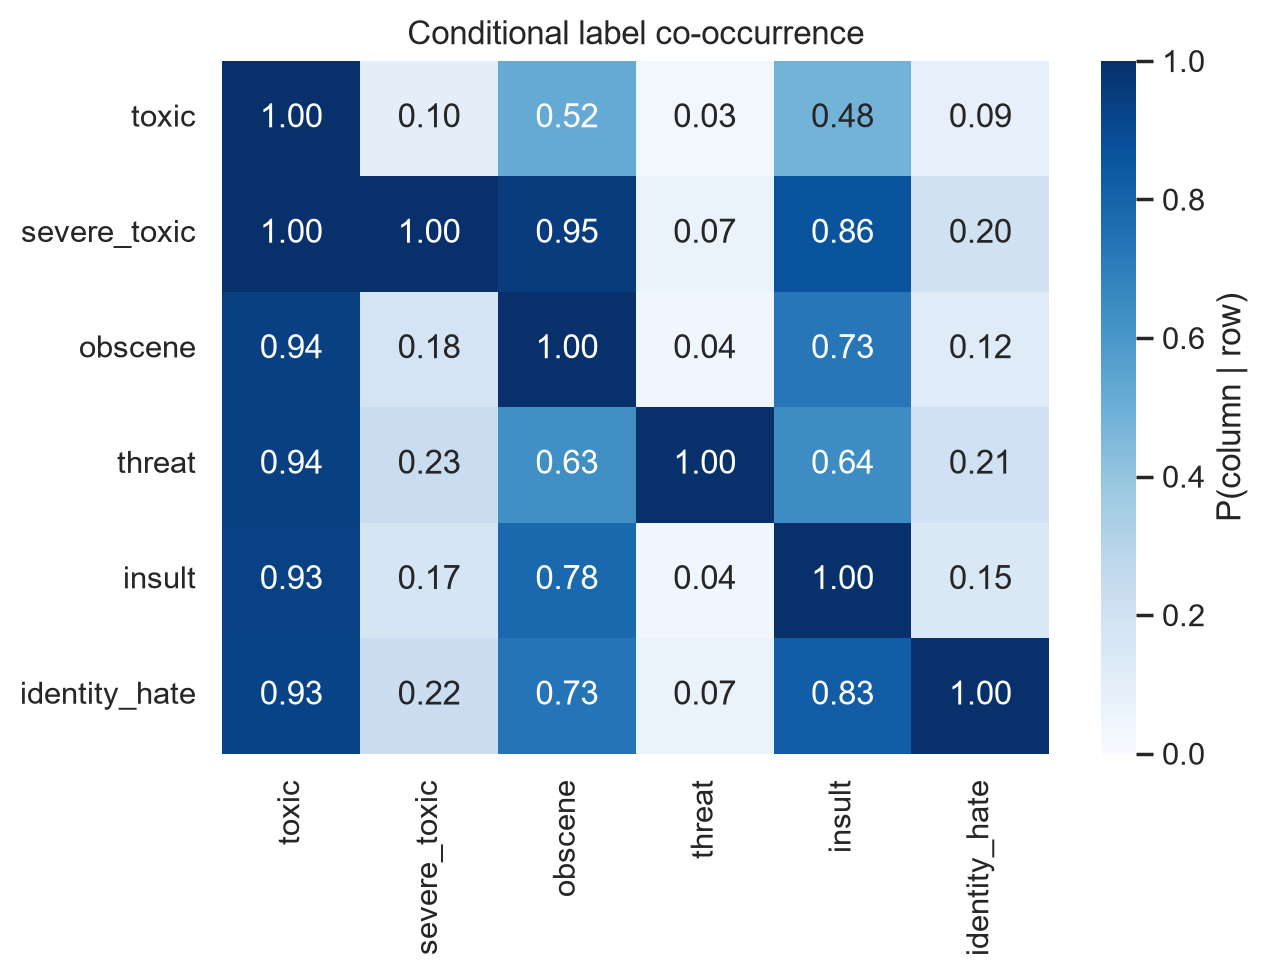
\includegraphics[width=0.6\linewidth]{label_cooccurrence}
  \caption{Conditional co-occurrence $P(\text{column} \mid \text{row})$.}
  \label{fig:cooc}
\end{figure}

\subsection{Comment length}

Comments are long-tailed (Figure~\ref{fig:length}): the median comment has 36
words, the 95th percentile 230 and the longest 1,411.  This informs the
transformer's maximum sequence length of 192 sub-word tokens, which keeps most
comments whole.

\begin{figure}[htbp]
  \centering
  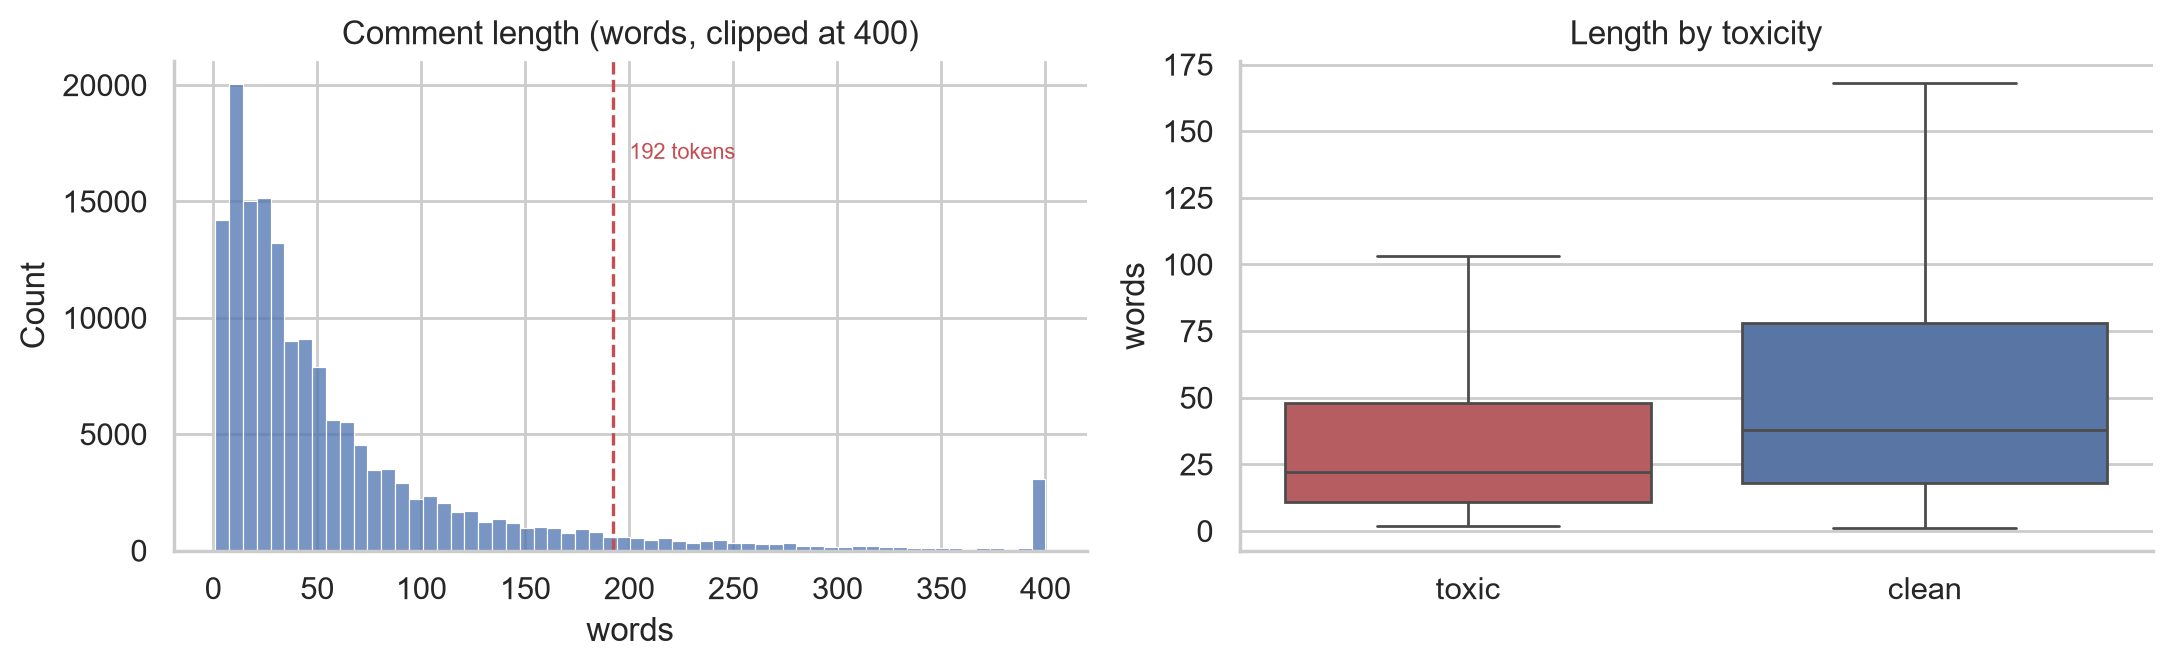
\includegraphics[width=0.95\linewidth]{comment_length}
  \caption{Distribution of comment length, and length by toxicity.}
  \label{fig:length}
\end{figure}

% =========================================================================== %
\section{Methodology}
% =========================================================================== %

Figure~\ref{fig:pipeline} summarises the system.  Two families of models turn
a comment into one score per label: linear classifiers over TF-IDF features,
and a fine-tuned transformer that reads the raw text.  A per-label threshold
then turns each score into a decision.

\begin{figure}[H]
  \centering
  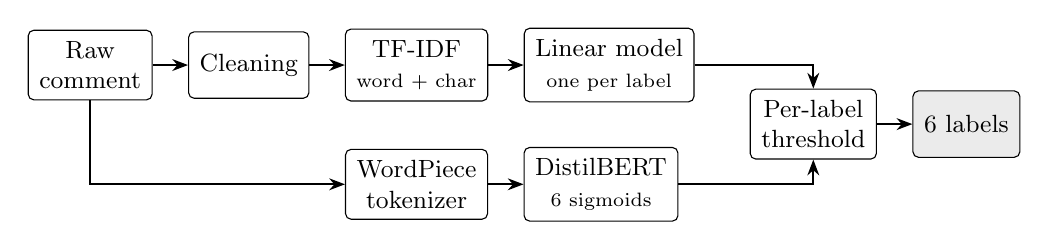
\begin{tikzpicture}[
      node distance=0.45cm and 0.45cm,
      box/.style={draw, rounded corners=2pt, align=center, font=\small,
                  minimum height=2.4em, inner sep=4pt},
      arrow/.style={-{Stealth[length=2mm]}, thick}]
    \node[box] (raw) {Raw\\comment};
    \node[box, right=of raw] (clean) {Cleaning};
    \node[box, right=of clean] (tfidf) {TF-IDF\\{\scriptsize word + char}};
    \node[box, right=of tfidf] (lin) {Linear model\\{\scriptsize one per label}};
    \node[box, below=0.6cm of tfidf] (tok) {WordPiece\\tokenizer};
    \node[box, right=of tok] (bert) {DistilBERT\\{\scriptsize 6 sigmoids}};
    \node[box, right=0.7cm of lin, yshift=-0.75cm] (thr) {Per-label\\threshold};
    \node[box, right=of thr, fill=black!8] (out) {6 labels};
    \draw[arrow] (raw) -- (clean);
    \draw[arrow] (clean) -- (tfidf);
    \draw[arrow] (tfidf) -- (lin);
    \draw[arrow] (raw) |- (tok);
    \draw[arrow] (tok) -- (bert);
    \draw[arrow] (lin.east) -| (thr.north);
    \draw[arrow] (bert.east) -| (thr.south);
    \draw[arrow] (thr) -- (out);
  \end{tikzpicture}
  \caption{Overview of the system.  Top: the classical pipeline; bottom: the
    transformer.  Thresholds are tuned on data from the training fold only.}
  \label{fig:pipeline}
\end{figure}

\subsection{Preprocessing}

The comments are raw wiki markup written by anonymous editors.  A configurable
cleaner, implemented as a scikit-learn transformer so that it runs inside each
fold, applies in order: removal of user signatures and escaped newlines;
replacement of URLs and IP addresses with placeholder tokens; lower-casing;
expansion of English contractions; reversal of common obfuscations
(\texttt{sh!t}, \texttt{b1tch}), where digits are rewritten only inside tokens
that also contain letters so that numbers survive; removal of punctuation; and
collapsing of character runs longer than two (\texttt{stuuuupid} $\to$
\texttt{stuupid}), which keeps the emphasis signal.  The transformer receives
the raw text, since its sub-word tokenizer handles casing and punctuation
itself.

\subsection{Models}

All models output a score in $[0,1]$ for each of the six labels.

\paragraph{Baselines.}
\emph{prior} predicts each label's training frequency for every comment; its
ROC-AUC is 0.5 by construction and it shows what accuracy-like metrics reward
on imbalanced data.  \emph{keyword} flags a comment when it contains a word
from a fixed profanity list: it is the rule-based system a team would build
without machine learning, and therefore the honest reference point for whether
learning is worth it.

\paragraph{Linear models.}
The three linear models share one feature space: the union of a word TF-IDF
(unigrams and bigrams, 50,000 features) and a character TF-IDF (2- to 5-grams
within word boundaries, 50,000 features).  A term $t$ in comment $d$ is
weighted by
\begin{equation}
  w_{t,d} = \bigl(1 + \log \mathit{tf}_{t,d}\bigr) \cdot \mathit{idf}_t,
  \qquad
  \mathit{idf}_t = \log\frac{1 + N}{1 + \mathit{df}_t} + 1,
\end{equation}
where $\mathit{tf}_{t,d}$ counts $t$ in $d$, $N$ is the number of training
comments and $\mathit{df}_t$ the number containing $t$; each vector is then
normalised to unit length.  The logarithm on the term frequency (``sublinear''
TF) stops a word repeated ten times from dominating the vector.  Character
n-grams are robust to the misspellings and obfuscations that dominate abusive
text: the pieces of \texttt{stuupid} survive even when the whole word is
spelt differently.  The vectorisers are fitted on the training fold only.

Following the binary-relevance approach, one binary classifier is fitted per
label.  All three compute a linear score $s(\mathbf{x}) = \mathbf{w}^\top
\mathbf{x} + b$ and differ in how $\mathbf{w}$ is learnt.  For a label with
targets $y_i \in \{0,1\}$ (or $\pm1$ for the SVM) and class weights $c_i$,
logistic regression and the linear SVM minimise respectively
\begin{equation}
  \frac{\lVert \mathbf{w} \rVert^2}{2C}
  + \sum_i c_i \Bigl[ -y_i \log \sigma(s_i) - (1-y_i)\log\bigl(1-\sigma(s_i)\bigr) \Bigr],
  \qquad
  \frac{\lVert \mathbf{w} \rVert^2}{2C} + \sum_i c_i \max(0,\, 1 - y_i s_i)^2,
\end{equation}
the L2-regularised log-loss and squared hinge loss, where $\sigma$ is the
logistic function and $C$ sets the strength of the regularisation.  The three
models are:
\begin{itemize}
  \item \emph{logreg}: logistic regression with balanced class weights
        ($C = 4$);
  \item \emph{linear\_svm}: a linear support vector machine with balanced
        class weights ($C = 0.5$), whose decision function is squashed through
        a sigmoid to obtain a score;
  \item \emph{nbsvm}: the NB-SVM of Wang and Manning~\cite{wang2012}, which
        multiplies the features by the Naive Bayes log-count ratio
        $r = \log\big(P(f \mid y{=}1) / P(f \mid y{=}0)\big)$ before fitting an
        unweighted logistic regression ($C = 4$); the rescaling itself already
        emphasises the features of the positive class.  It was a popular and
        strong baseline in the competition.
\end{itemize}
Balanced class weights scale each class inversely to its frequency: for
\emph{threat}, a positive example weighs about 330 times as much as a negative
one.

\paragraph{Transformer.}
\emph{distilbert} fine-tunes DistilBERT~\cite{sanh2019}
(\texttt{distilbert-base-uncased}), a version of BERT compressed by knowledge
distillation: 6 transformer layers instead of 12, hidden size 768, 12
attention heads and 66 million parameters, 40\% smaller and 60\% faster than
BERT-base while retaining 97\% of its score on the GLUE benchmark.  A comment
is split into WordPiece sub-word tokens, prefixed with a \texttt{[CLS]} token
and truncated to 192 tokens.  Self-attention lets every token's
representation depend on the whole comment, which is what can separate
``this article is garbage'' from ``you are garbage''.  The final
representation of \texttt{[CLS]} feeds a new classification head with six
outputs $z_k$, one per label, each passed through a sigmoid, $p_k =
\sigma(z_k)$.  Because the labels are not mutually exclusive, the head uses
six independent sigmoids rather than a softmax, and the loss is the binary
cross-entropy summed over the labels,
\begin{equation}
  \mathcal{L} = -\sum_{k=1}^{6} \bigl[\, y_k \log p_k + (1-y_k)\log(1-p_k) \bigr].
\end{equation}
The whole network is trained for two epochs with AdamW (learning rate
$3\cdot10^{-5}$, weight decay 0.01), batch size 32, gradient clipping at 1.0
and mixed precision, on an NVIDIA RTX 4050 laptop GPU with 6\,GB of memory.
The loss is not class-weighted, which matters for the thresholds
(Section~\ref{sec:thresholds}).

\subsection{Cross validation}

Plain stratified $k$-fold is defined for a single target.  We use
\emph{iterative stratification}~\cite{sechidis2011}, which assigns comments to
folds so that the frequency of every label, including the rare ones, is
balanced across folds.  We use $k = \NFolds$, and all models are evaluated on
the \emph{same} fold assignment, which makes a paired comparison of their
per-fold scores valid.

\subsection{Threshold tuning}

Turning scores into labels needs a threshold per label.  Instead of the default
0.5, we choose the threshold that maximises F1 on an inner hold-out of 15\% of
each \emph{training} fold; the model is fitted on the remaining 85\%.  The
validation fold is never used to choose a threshold, so the reported F1 is not
optimistically biased.

\subsection{Metrics}

\begin{itemize}
  \item \textbf{Mean column-wise ROC-AUC}, the competition's official metric:
        the ROC-AUC of each label, averaged.  It is threshold-free and
        insensitive to class imbalance.
  \item \textbf{PR-AUC} (average precision) per label and averaged.  On a label
        with a 0.3\% positive rate, ROC-AUC is dominated by the easy negatives;
        PR-AUC measures how precise the model is on the positives, and is the
        more discriminating metric for rare labels.
  \item \textbf{Macro F1} (unweighted mean over labels, so rare labels count as
        much as frequent ones) and \textbf{micro F1} (pooled over all
        label decisions), at the tuned thresholds.
  \item \textbf{Hamming loss} and \textbf{subset accuracy}, the standard
        multi-label metrics, computed for every fold and stored in
        \texttt{results/} for completeness.
\end{itemize}

\subsection{Statistical comparison}

For each pair of models we apply the Wilcoxon signed-rank test to their
per-fold mean column-wise AUCs, with a Bonferroni correction for the number of
pairs.  With five folds the smallest attainable two-sided p-value is
$2/2^5 = 0.0625$, reached when one model wins on every fold; no pairwise
difference can therefore be significant at the 5\% level, and we report the
consistency of the ranking across folds alongside the p-values.

% =========================================================================== %
\section{Implementation}
% =========================================================================== %

The application is written in Python and organised as a package
(\texttt{src/}) used by command-line scripts and by three Jupyter notebooks,
which also run on Google Colab.

\begin{itemize}
  \item \texttt{dataio}: loading and schema validation of the Kaggle files, and
        a synthetic generator used to smoke-test the pipeline without the data.
  \item \texttt{preprocessing}: the text cleaner and the TF-IDF vectorisers.
  \item \texttt{models}: a common \texttt{fit}/\texttt{predict\_proba}
        interface implemented by every model, and a registry that builds a
        model from its name.
  \item \texttt{evaluation}: multi-label folds, cross validation, metrics,
        threshold optimisation, statistical tests, the hierarchy check and the
        bias audit.
  \item \texttt{repository}: persistence of datasets and results behind one
        interface with two implementations, file system and in memory
        (Section~\ref{sec:persistence}).
\end{itemize}

\subsection{Persistence layer}
\label{sec:persistence}

The course requires that data can be managed both in memory and through files,
and that switching between the two leaves the classes, their methods and the
business logic unchanged.  We meet this with the \emph{repository} pattern.
Two abstract base classes define what can be done with stored data, without
saying where it is stored:

\begin{lstlisting}
class DatasetRepository(ABC):          # tabular data (pandas.DataFrame)
    def save(self, name: str, frame: pd.DataFrame) -> None: ...
    def load(self, name: str) -> pd.DataFrame: ...
    def exists(self, name: str) -> bool: ...
    def list_datasets(self) -> list[str]: ...
    def delete(self, name: str) -> None: ...

class ArtifactRepository(ABC):         # results: metrics, scores, models
    def save(self, name: str, obj: Any) -> None: ...
    def load(self, name: str) -> Any: ...
    def exists(self, name: str) -> bool: ...
    def list_artifacts(self) -> list[str]: ...
    def delete(self, name: str) -> None: ...
\end{lstlisting}

Each has two implementations.  The file-system ones write CSV or Parquet files
for datasets, and JSON (or \texttt{joblib} for objects JSON cannot represent)
for artifacts; the in-memory ones keep the objects in a dictionary and return
deep copies of data frames and of plain containers, so that a caller cannot
mutate stored data by accident.  A factory is the
only code that names a concrete class:

\begin{lstlisting}
def get_dataset_repository(config) -> DatasetRepository:
    if config.persistence_backend == "memory":
        return _MEMORY_DATASETS              # process-wide singleton
    return FileDatasetRepository(root=config.processed_dir)
\end{lstlisting}

Every other module -- the data loader, the experiment runner, the report
scripts, the notebooks -- obtains its repository from the factory and is typed
against the abstract interface only.  Switching the whole application between
the two layers is therefore a single value: the \texttt{persistence\_backend}
field of the configuration, the \texttt{TCC\_PERSISTENCE} environment
variable, or the \texttt{--backend file|memory} flag of the experiment
scripts.  The repository tests are parametrised to run unchanged against both
implementations, and the suite includes a
test that executes one piece of business logic under each backend and checks
that the results are identical.  In practice we use the memory backend for
quick notebook sessions and for the tests, and the file backend for the
experiments, whose results must outlive the process.

\texttt{scripts/run\_experiment.py} runs the cross validation and stores every
artifact (per-fold metrics, out-of-fold scores, thresholds, significance
matrix, bias audit) in \texttt{results/}.  Because the transformer needs a
GPU, it is run separately, and \texttt{scripts/merge\_runs.py} folds its
results into the main run after checking that both used the same folds.  The
tables and figures of this report are generated from those files by two
scripts, never copied by hand.
A test suite of 80 \texttt{pytest} tests covers the data layer, the
preprocessing, the models, the metrics, the cross validation and both
persistence backends.

% =========================================================================== %
\section{Results}
% =========================================================================== %

This section and the next two answer the research questions in turn: the
model comparison and its cost answer RQ1
(Sections~
ef{sec:comparison} and~
ef{sec:cost}); the per-label results,
the thresholds and the label hierarchy answer RQ2
(Sections~
ef{sec:perlabel}, 
ef{sec:thresholds} and~
ef{sec:hierarchy});
the official test set and the significance tests answer RQ3
(Sections~
ef{sec:testset} and~
ef{sec:significance}); and the error and
bias analyses answer RQ4 (Sections~
ef{sec:errors} and~
ef{sec:bias}).

\subsection{Model comparison (RQ1)}
\label{sec:comparison}

Table~\ref{tab:leaderboard} and Figure~\ref{fig:leaderboard} rank the models by
the official metric.

\begin{table}[H]
  \centering
  \caption{Cross-validated results, mean over \NFolds{} folds ($\pm$ standard
    deviation for AUC).  F1 at the tuned thresholds.  Fit time per fold.}
  \label{tab:leaderboard}
  % Generated by scripts/make_report_assets.py -- do not edit.
% Re-run the script instead; every number here comes from results/.

\begin{tabular}{lccccr}
  \toprule
  Model & Mean col.\ AUC & PR-AUC & Macro $F_1$ & Micro $F_1$ & Fit (s) \\
  \midrule
  distilbert & 0.9898 $\pm$ 0.0011 & 0.7193 & 0.6827 & 0.7870 & 2238.4 \\
  logreg & 0.9841 $\pm$ 0.0010 & 0.6726 & 0.6410 & 0.7551 & 232.0 \\
  nbsvm & 0.9830 $\pm$ 0.0010 & 0.6665 & 0.6350 & 0.7566 & 238.0 \\
  linear\_svm & 0.9800 $\pm$ 0.0008 & 0.6559 & 0.6306 & 0.7486 & 203.8 \\
  keyword & 0.7831 $\pm$ 0.0075 & 0.1298 & 0.2485 & 0.2821 & 0.6 \\
  prior & 0.5000 $\pm$ 0.0000 & 0.0367 & 0.0616 & 0.1231 & 0.0 \\
  \bottomrule
\end{tabular}

\end{table}

\begin{figure}[H]
  \centering
  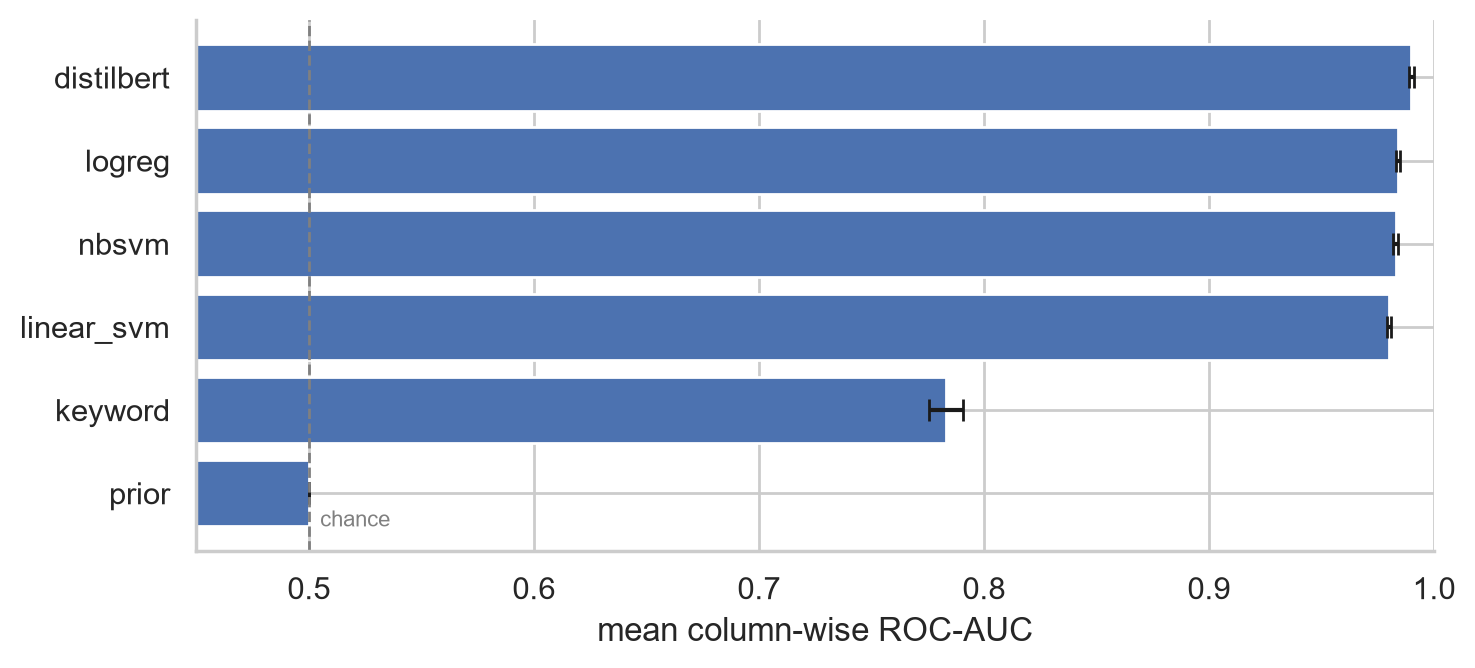
\includegraphics[width=0.75\linewidth]{leaderboard}
  \caption{Mean column-wise ROC-AUC per model, with the standard deviation over
    folds.}
  \label{fig:leaderboard}
\end{figure}

Four observations stand out.

\emph{Learning is worth it.}  The keyword baseline reaches an AUC of 0.78 but a
macro F1 of only 0.25; every learned model exceeds 0.98 AUC and 0.63 macro F1.
The prior baseline sits at exactly 0.5 AUC, as expected.

\emph{The transformer is the best model on every metric.}  DistilBERT reaches
\BestAUC{} AUC against \RunnerUpAUC{} for the best linear model, and it wins on
each of the five folds (fold AUCs 0.9889--0.9916 against 0.9827--0.9850).  The
gain is larger where it matters most: macro F1 rises from 0.641 to 0.683 and
mean PR-AUC from 0.673 to 0.719, mainly through the rare labels
(Section~\ref{sec:perlabel}).

\emph{Among the linear models the differences are small but consistent.}
logreg leads with 0.9841, ahead of nbsvm (0.9830) and linear\_svm (0.9800).
The gap between logreg and nbsvm is only 0.001 AUC, yet logreg wins on all five
folds.  In our feature space, which already includes character n-grams, the NB
rescaling brings no gain.

\emph{All learned models are close to the competition's best.}  The winning
private-leaderboard score was about 0.988, obtained with large ensembles of
deep models.  In cross validation a single logistic regression comes within
0.005 of it and a single DistilBERT matches it, but cross validation is
optimistic: on the official test set the logistic regression scores 0.9784
(Section~\ref{sec:testset}).

\subsection{Per-label results (RQ2)}
\label{sec:perlabel}

The aggregate AUC hides how unequal the labels are
(Table~\ref{tab:perlabel}, Figure~\ref{fig:prauc}).  For DistilBERT, ROC-AUC
is above 0.98 on every label, but PR-AUC ranges from 0.92 on \emph{obscene} and
\emph{toxic} to 0.50 on \emph{severe\_toxic}, 0.54 on \emph{threat} and 0.61 on
\emph{identity\_hate}.  The frequent, lexically marked labels are easy; the rare
ones are hard both because they have few training examples and because they
depend on meaning rather than vocabulary -- a threat need not contain a single
offensive word, and \emph{severe\_toxic} differs from \emph{toxic} by degree.
The transformer's largest gains over logreg are on two of these rare labels:
+0.11 PR-AUC on \emph{identity\_hate} and +0.05 on \emph{severe\_toxic},
against +0.015 to +0.036 on the other four.

\begin{table}[H]
  \centering
  \caption{Per-label results of \BestModel, mean over folds.  Support is the
    number of positives per validation fold.}
  \label{tab:perlabel}
  % Generated by scripts/make_report_assets.py -- do not edit.
% Re-run the script instead; every number here comes from results/.

\begin{tabular}{lrccccccc}
  \toprule
  Label & Support & ROC-AUC & PR-AUC & Prec. & Recall & $F_1$ & Thresh. \\
  \midrule
  toxic & 3{,}059 & 0.9861 & 0.9160 & 0.8357 & 0.8283 & 0.8317 & 0.494 \\
  severe\_toxic & 319 & 0.9914 & 0.4998 & 0.4408 & 0.6395 & 0.5193 & 0.265 \\
  obscene & 1{,}690 & 0.9936 & 0.9185 & 0.8378 & 0.8416 & 0.8391 & 0.482 \\
  threat & 96 & 0.9901 & 0.5374 & 0.5413 & 0.5919 & 0.5637 & 0.255 \\
  insult & 1{,}575 & 0.9887 & 0.8296 & 0.7281 & 0.8060 & 0.7648 & 0.414 \\
  identity\_hate & 281 & 0.9890 & 0.6145 & 0.5591 & 0.6028 & 0.5778 & 0.380 \\
  \bottomrule
\end{tabular}

\end{table}

\begin{figure}[H]
  \centering
  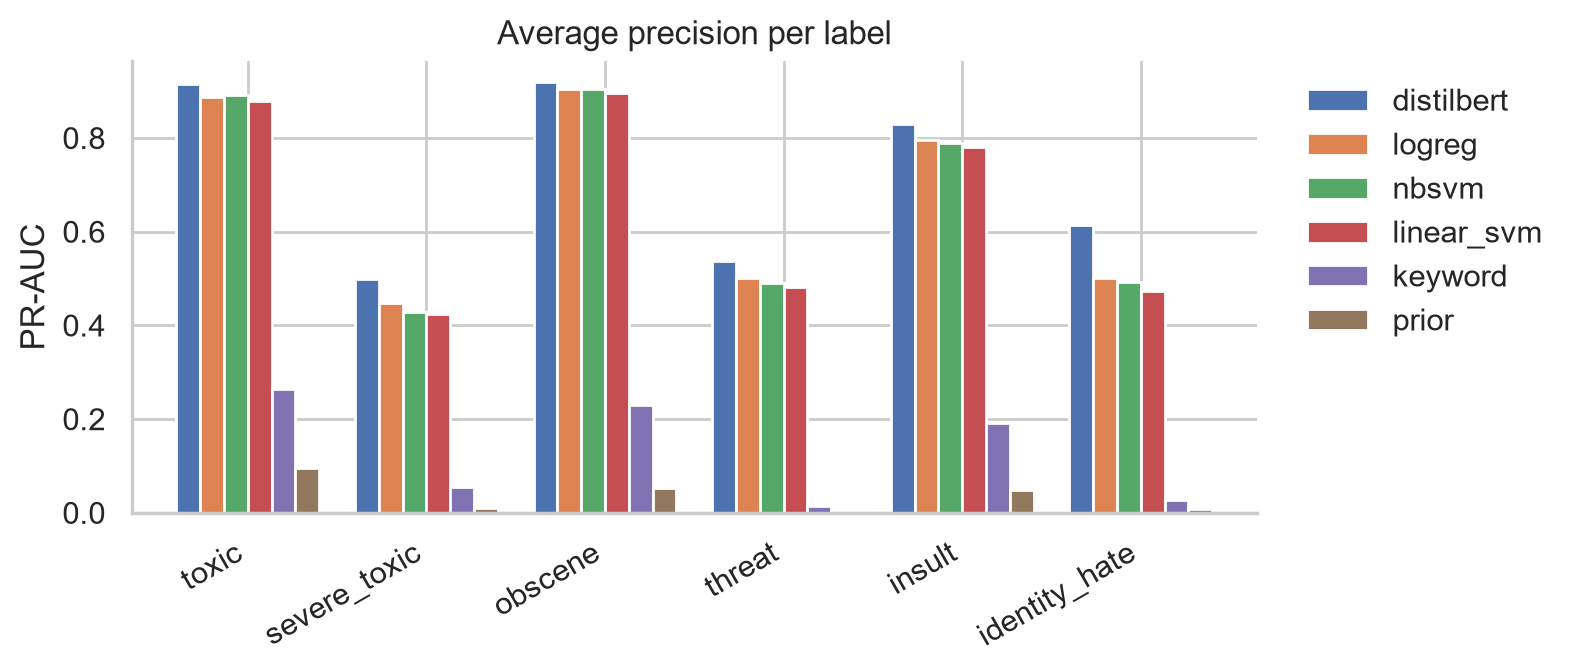
\includegraphics[width=0.85\linewidth]{pr_auc_per_label}
  \caption{PR-AUC per label and model.}
  \label{fig:prauc}
\end{figure}

\subsection{Effect of threshold tuning (RQ2)}
\label{sec:thresholds}

Table~\ref{tab:thresholds} compares F1 at the default cut-off of 0.5 with F1 at
the tuned threshold.  For DistilBERT the tuned thresholds lie \emph{below} 0.5,
between 0.25 and 0.49, and they matter a great deal on the rare labels: +0.17
F1 on \emph{severe\_toxic} and +0.11 on \emph{threat}.  Trained with an
unweighted loss, the transformer is cautious about rare labels and its scores
for them tend to stay below 0.5; the tuned threshold corrects this.

Logistic regression and the linear SVM behave in the opposite way.  They are
trained with balanced class weights, which inflate the scores of the positive
class: logreg's tuned
thresholds lie between 0.60 and 0.75, and tuning gains only $-0.006$ to
$+0.023$ F1, because the class weights have already done most of the
correction.  Threshold tuning and class weighting are thus two answers to the
same imbalance, and one of them is necessary.

\begin{table}[H]
  \centering
  \caption{F1 of \BestModel{} at 0.5 and at the tuned threshold.}
  \label{tab:thresholds}
  % Generated by scripts/make_report_assets.py -- do not edit.
% Re-run the script instead; every number here comes from results/.

\begin{tabular}{lcccc}
  \toprule
  Label & Tuned thresh. & $F_1$ @ 0.5 & $F_1$ @ tuned & Gain \\
  \midrule
  toxic & 0.494 & 0.8291 & 0.8317 & $+$0.0026 \\
  severe\_toxic & 0.265 & 0.3459 & 0.5193 & $+$0.1734 \\
  obscene & 0.482 & 0.8379 & 0.8391 & $+$0.0013 \\
  threat & 0.255 & 0.4548 & 0.5637 & $+$0.1089 \\
  insult & 0.414 & 0.7491 & 0.7648 & $+$0.0157 \\
  identity\_hate & 0.380 & 0.5666 & 0.5778 & $+$0.0113 \\
  \bottomrule
\end{tabular}

\end{table}

\begin{figure}[H]
  \centering
  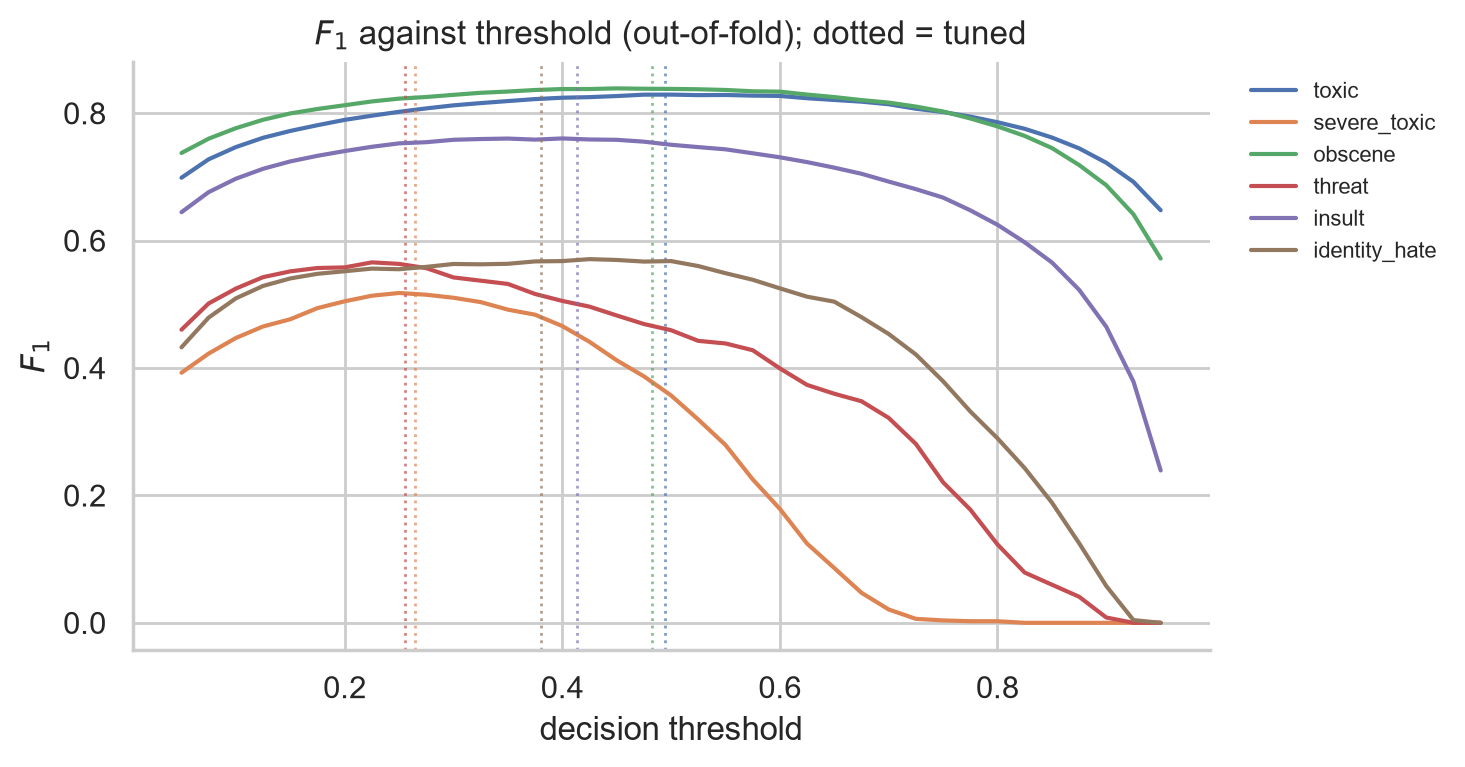
\includegraphics[width=0.8\linewidth]{threshold_sweep}
  \caption{F1 as a function of the decision threshold, out-of-fold scores.}
  \label{fig:sweep}
\end{figure}

\subsection{Official test set (RQ3)}
\label{sec:testset}

Cross validation compares models with each other; it does not say how a model
would have fared in the competition.  For that we scored the models once on
the 63,978 test comments that Kaggle labelled after the competition closed
(\texttt{scripts/evaluate\_test\_set.py}).  Each model is trained as in one
fold: fitted on 85\% of the full training set, with its thresholds tuned on
the remaining 15\%.  The transformer was not re-trained for this experiment,
since that needs another GPU run.

\begin{table}[H]
  \centering
  \caption{Results on the scored part of the official test set.}
  \label{tab:testset}
  % Generated by scripts/make_report_assets.py -- do not edit.
% Re-run the script instead; every number here comes from results/.

\begin{tabular}{lcccc}
  \toprule
  Model & Mean col.\ AUC & PR-AUC & Macro $F_1$ & Micro $F_1$ \\
  \midrule
  logreg & 0.9784 & 0.6098 & 0.5763 & 0.6486 \\
  nbsvm & 0.9781 & 0.6003 & 0.5573 & 0.6370 \\
  linear\_svm & 0.9746 & 0.5933 & 0.5507 & 0.6348 \\
  keyword & 0.7815 & 0.1131 & 0.2177 & 0.2450 \\
  prior & 0.5000 & 0.0378 & 0.0641 & 0.1280 \\
  \bottomrule
\end{tabular}

\end{table}

The ranking of the models is the same as in cross validation, but every
learned model scores lower: logreg reaches 0.9784 AUC on the test set against
0.9841 in cross validation, and the other linear models lose about 0.005 as
well.  Macro F1 drops more (0.641 to 0.576 for logreg), because thresholds
tuned on training data transfer imperfectly to the test comments.  Cross
validation on the training set is thus optimistic for this task, and the gap
between our best linear model and the winning private-leaderboard score
(about 0.988) is 0.010 rather than the 0.005 that the cross-validated number
suggests.

\subsection{Statistical significance (RQ3)}
\label{sec:significance}

Table~\ref{tab:significance} gives the pairwise Wilcoxon p-values.  Every pair
reaches the minimum attainable value of 0.0625: for each pair of models, one of
the two is better on all five folds.  The ranking is thus perfectly consistent
across folds, but with five folds this cannot be declared significant at the
5\% level, let alone at the Bonferroni-corrected level of $0.05/15 = 0.0033$.
Establishing significance would require more folds or repeated cross
validation.

\begin{table}[H]
  \centering
  \caption{Pairwise Wilcoxon signed-rank p-values on the per-fold mean
    column-wise AUC.  Bold: significant at the Bonferroni-corrected level.}
  \label{tab:significance}
  % Generated by scripts/make_report_assets.py -- do not edit.
% Re-run the script instead; every number here comes from results/.

\begin{tabular}{lcccccc}
  \toprule
  Model & prior & keyword & logreg & nbsvm & linear\_svm & distilbert \\
  \midrule
  prior & --- & 0.062 & 0.062 & 0.062 & 0.062 & 0.062 \\
  keyword & 0.062 & --- & 0.062 & 0.062 & 0.062 & 0.062 \\
  logreg & 0.062 & 0.062 & --- & 0.062 & 0.062 & 0.062 \\
  nbsvm & 0.062 & 0.062 & 0.062 & --- & 0.062 & 0.062 \\
  linear\_svm & 0.062 & 0.062 & 0.062 & 0.062 & --- & 0.062 \\
  distilbert & 0.062 & 0.062 & 0.062 & 0.062 & 0.062 & --- \\
  \bottomrule
\end{tabular}

\end{table}

\subsection{Cost against accuracy (RQ1)}
\label{sec:cost}

Figure~\ref{fig:cost} relates accuracy to training cost.  The three linear
models train in 3.5--4 minutes per fold on a laptop CPU, about 400 times the
cost of the keyword rule but still cheap enough to retrain daily.  DistilBERT
needs 37 minutes per fold on average on a laptop GPU (an NVIDIA RTX 4050 with
mixed precision), about ten times as long; individual folds took between 19
and 82 minutes.  The 0.006 AUC it gains costs
an order of magnitude more compute and a GPU; whether that is worth it depends
on how much the rare labels matter to the application.

The two families were timed in separate runs on different machines -- the
linear models on a laptop CPU, the transformer on a laptop GPU -- so the ratio
is indicative only.

\begin{figure}[H]
  \centering
  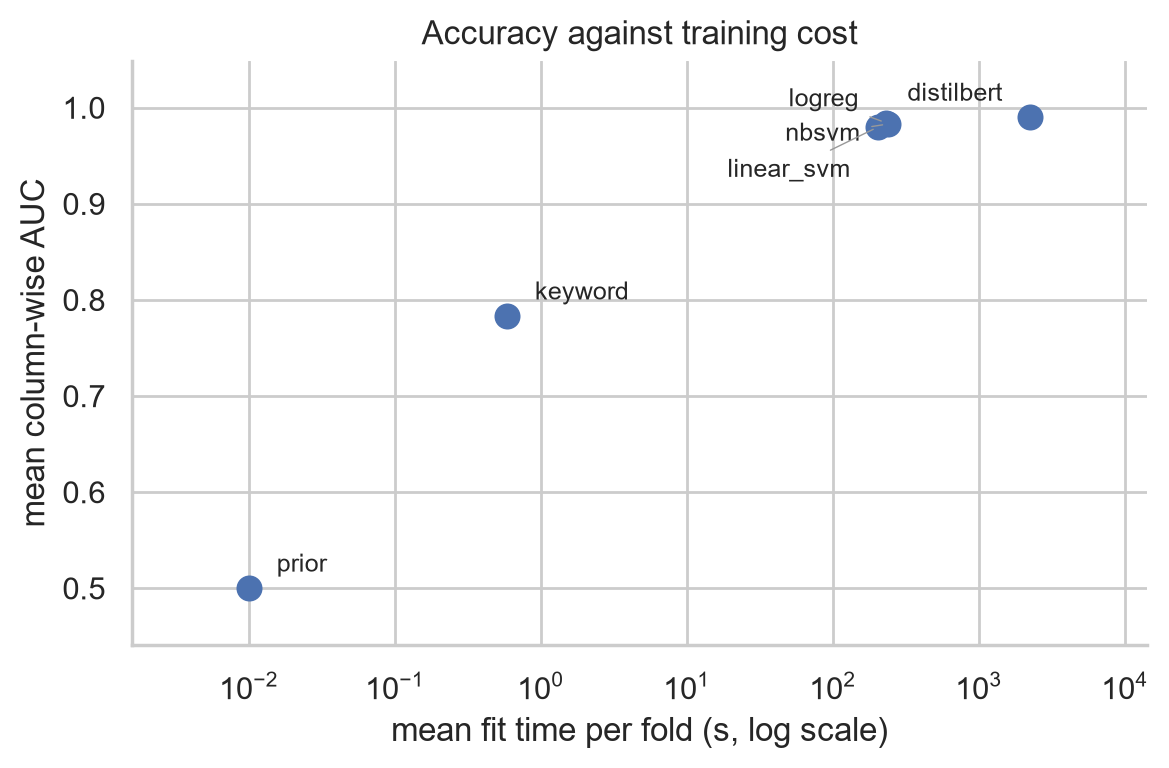
\includegraphics[width=0.65\linewidth]{cost_vs_accuracy}
  \caption{Mean column-wise AUC against fit time per fold (log scale).}
  \label{fig:cost}
\end{figure}

% =========================================================================== %
\section{Error analysis (RQ4)}
\label{sec:errors}
% =========================================================================== %

\subsection{Confusion matrices}

Figure~\ref{fig:confusion} shows the confusion matrix of each label at its
tuned threshold, pooled over the out-of-fold predictions of DistilBERT.  On
\emph{toxic} it makes 2,500 false positives and 2,626 false negatives out of
15,294 toxic comments, against 2,766 and 3,301 for logreg.

\begin{figure}[H]
  \centering
  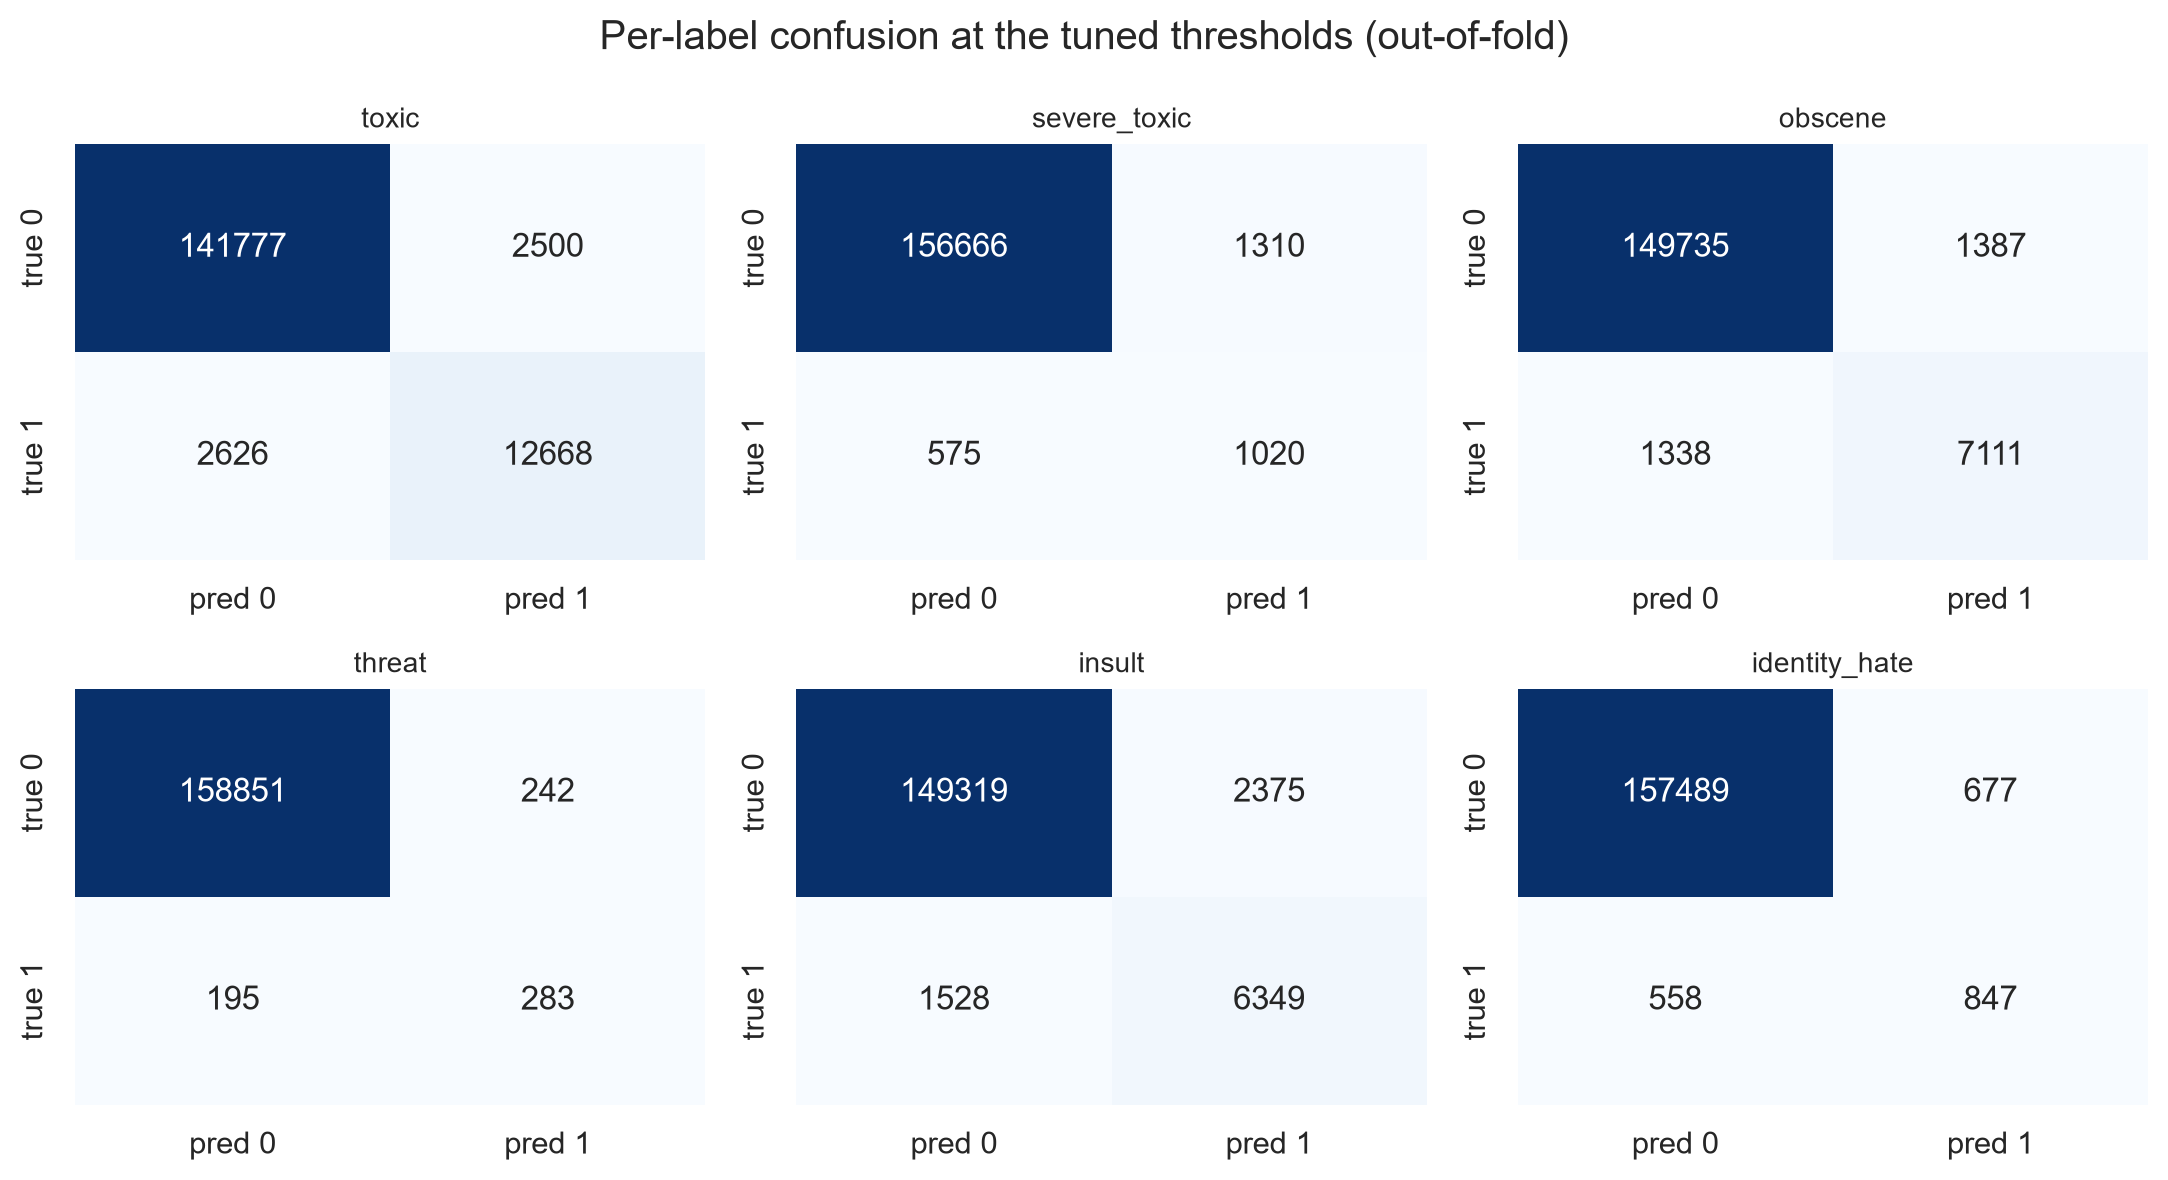
\includegraphics[width=0.95\linewidth]{confusion_matrices}
  \caption{Confusion matrices at the tuned thresholds, out-of-fold.}
  \label{fig:confusion}
\end{figure}

\subsection{Error taxonomy}

We read the false positives and false negatives on \emph{toxic} that each of
logreg and DistilBERT was most confident about
(\texttt{scripts/make\_error\_examples.py}), and compared the two models'
scores on the same comments.  The errors fall into a few recurring categories.

\paragraph{False positives (clean comments flagged as toxic).}
\begin{itemize}
  \item \emph{Annotation noise.}  Most of the confident ``errors'' of both
        models are plainly abusive comments -- direct personal insults, often
        with slurs (``you're an asshole and that's all there is to it'') --
        that the annotators left unlabelled.  Here the model is right and the
        label is wrong.  For DistilBERT, ten of its twelve most confident
        false positives are of this kind.
  \item \emph{Profanity without abuse.}  Swear words used descriptively or
        about oneself.  A list of TV content ratings quoting the words they
        warn about scores 1.00 under logreg but 0.45 under DistilBERT, which
        is below its threshold: reading the context, the transformer
        recognises the quotation.  A comment about oneself (``I'm going
        through deep shit'') still fools both (1.00 and 0.83).
  \item \emph{Mild incivility.}  Rude but borderline comments (``It must suck
        to be you then'') on which annotators disagree.
\end{itemize}

\paragraph{False negatives (toxic comments missed).}
\begin{itemize}
  \item \emph{Annotation noise.}  Comments with no hostility at all -- a list
        of a band's musical influences, a note about magazine-cover images --
        are labelled toxic.  Both models score them near zero, rightly.
  \item \emph{Shouting and heated disagreement.}  Comments written in capitals
        or accusing other editors, with no offensive vocabulary
        (``STOP DELETING MY ADDITION!'').  Both models miss them (0.00 and
        0.04).
  \item \emph{Sarcasm.}  ``Thanks for participating in the conspiracy against
        me.''  The words are polite and the intent is not; both models score
        it 0.00.
  \item \emph{Harassment without profanity, and toxicity diluted by length.}
        A sexual remark about a named person in innocuous words, or a short
        insult followed by a long pasted article.  DistilBERT raises these
        from about 0.00 under logreg to 0.17--0.20, but not above its
        threshold.
\end{itemize}

The transformer's advantage is visible in exactly the categories that depend
on context: who a swear word is aimed at, whether a sentence is a quotation.
Sarcasm and shouting remain beyond both models.  And a large share of the
remaining confident errors are labelling mistakes, which bound the score that
any model can reach on this data.

\subsection{Label hierarchy violations (RQ2)}
\label{sec:hierarchy}

The linear models predict each label independently, so nothing prevents them
from predicting a sub-type without \emph{toxic}.  logreg does so for 4 of its
2,503 \emph{severe\_toxic} predictions -- outputs that are impossible, since
the label never occurs without \emph{toxic} -- and for about 7\% of its
\emph{threat} and \emph{identity\_hate} predictions, close to the 6--7\% at
which these labels occur without \emph{toxic} in the data.

DistilBERT shares one encoder across the six outputs, and it behaves
differently (Table~\ref{tab:hierarchy}): it never predicts \emph{severe\_toxic}
or \emph{insult} without \emph{toxic}, and does so for at most 0.4\% of the
other sub-labels.  It has thus learnt the hierarchy -- and in fact
over-learnt it, since in the data 6--7\% of the \emph{obscene}, \emph{threat},
\emph{insult} and \emph{identity\_hate} comments are \emph{not} labelled toxic.
For the linear models, a post-processing rule that sets \emph{toxic} whenever
\emph{severe\_toxic} is predicted would remove the impossible outputs.

\begin{table}[H]
  \centering
  \caption{Predicted positives of each sub-label that lack a \emph{toxic}
    prediction, \BestModel, out-of-fold.}
  \label{tab:hierarchy}
  % Generated by scripts/make_report_assets.py -- do not edit.
% Re-run the script instead; every number here comes from results/.

\begin{tabular}{lrrr}
  \toprule
  Label & Predicted positive & Without \emph{toxic} & Rate \\
  \midrule
  severe\_toxic & 2{,}330 & 0 & 0.00\% \\
  obscene & 8{,}498 & 13 & 0.15\% \\
  threat & 525 & 2 & 0.38\% \\
  insult & 8{,}724 & 0 & 0.00\% \\
  identity\_hate & 1{,}524 & 4 & 0.26\% \\
  \bottomrule
\end{tabular}

\end{table}

% =========================================================================== %
\section{Unintended bias (RQ4)}
\label{sec:bias}
% =========================================================================== %

A model trained on this corpus sees identity terms mostly in abusive contexts
and can learn to penalise the term itself.  We measure this as follows: for
each identity term, we take the clean comments that mention it and compute the
false-positive rate of \emph{toxic} at the tuned threshold; dividing by the
false-positive rate on all clean comments gives a ratio that is 1 for an
unbiased model.

\begin{table}[H]
  \centering
  \caption{False-positive rate on \emph{toxic} for clean comments mentioning
    each identity term, against the background rate (\BestModel, out-of-fold).}
  \label{tab:bias}
  % Generated by scripts/make_report_assets.py -- do not edit.
% Re-run the script instead; every number here comes from results/.

\begin{tabular}{lrcccccc}
  \toprule
  Term & $n$ & Toxic rate & Subgroup FPR & Background FPR & Ratio & Subgroup AUC \\
  \midrule
  gay & 1{,}002 & 0.547 & 0.117 & 0.017 & 6.77 & 0.953 \\
  lesbian & 79 & 0.304 & 0.109 & 0.018 & 6.23 & 0.939 \\
  transgender & 31 & 0.194 & 0.080 & 0.018 & 4.56 & 0.973 \\
  black & 1{,}458 & 0.123 & 0.043 & 0.017 & 2.48 & 0.953 \\
  muslim & 744 & 0.105 & 0.030 & 0.017 & 1.72 & 0.946 \\
  white & 1{,}512 & 0.120 & 0.029 & 0.017 & 1.68 & 0.965 \\
  woman & 543 & 0.125 & 0.025 & 0.018 & 1.44 & 0.956 \\
  jewish & 763 & 0.092 & 0.025 & 0.018 & 1.40 & 0.955 \\
  christian & 1{,}175 & 0.067 & 0.020 & 0.018 & 1.14 & 0.963 \\
  female & 396 & 0.096 & 0.020 & 0.018 & 1.11 & 0.974 \\
  immigrant & 104 & 0.106 & 0.000 & 0.018 & 0.00 & 0.992 \\
  \bottomrule
\end{tabular}

\end{table}

\begin{figure}[H]
  \centering
  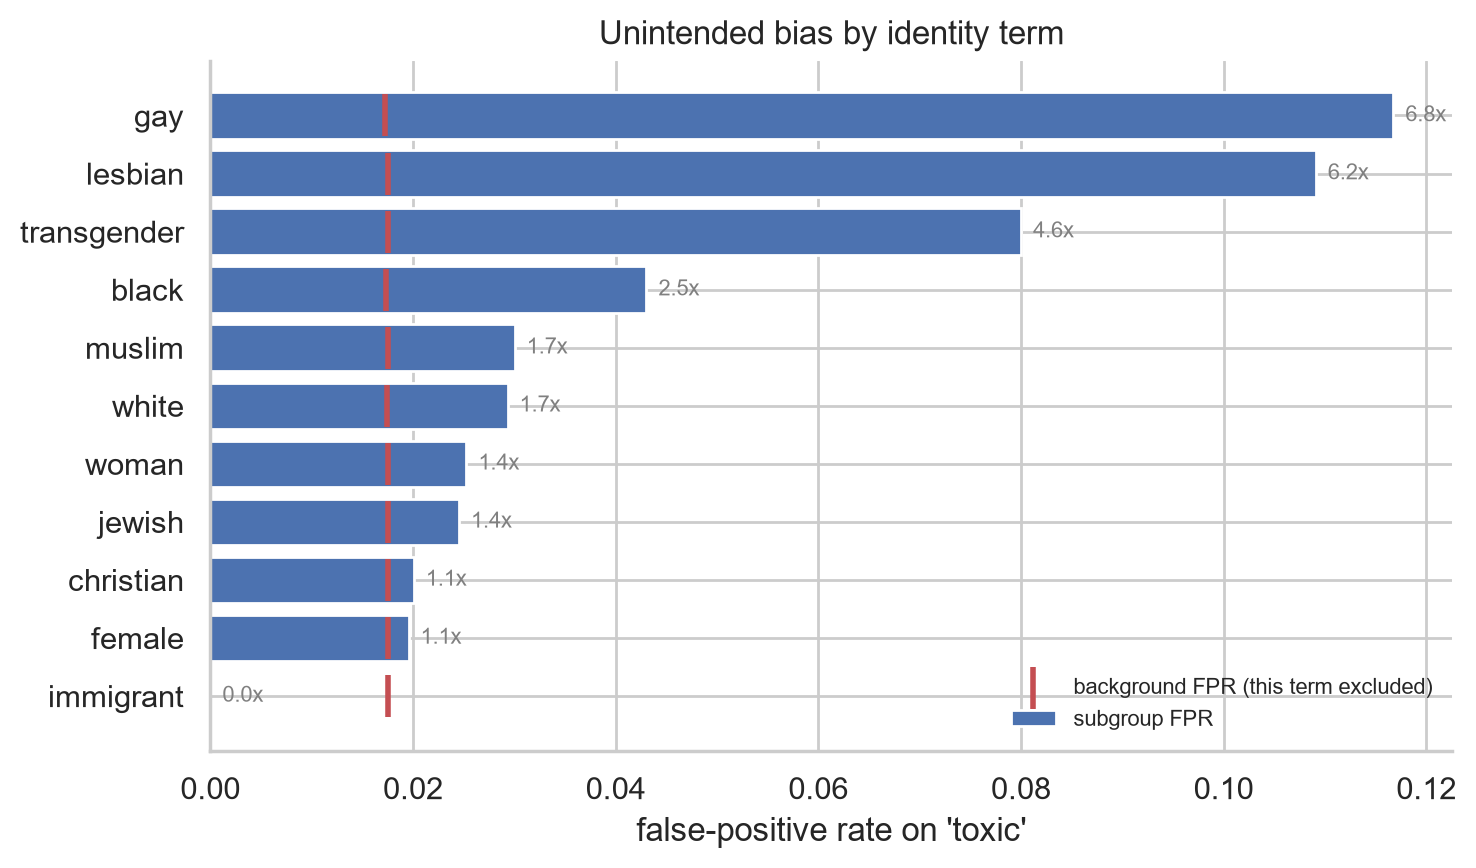
\includegraphics[width=0.75\linewidth]{identity_bias}
  \caption{False-positive rate on \emph{toxic} for clean comments mentioning
    each term (bars), against the background rate (red marks), with the ratio
    of the two; \BestModel, out-of-fold.}
  \label{fig:bias}
\end{figure}

The bias is large (Table~\ref{tab:bias}, Figure~\ref{fig:bias}).  For
DistilBERT, a clean comment mentioning \emph{gay} is flagged as toxic 6.8
times as often as the average clean comment, \emph{lesbian} 6.2 times,
\emph{transgender} 4.6 times (on only 31 comments) and \emph{black} 2.5 times.
The cause is visible in the data: 55\% of the comments mentioning \emph{gay}
are toxic, against 10\% overall, so the term itself is a strong predictor.
The subgroup AUC stays high (0.94--0.99), which means the model still ranks
toxic above non-toxic comments \emph{within} each group; the problem is that
the whole group is shifted upwards.

The bag-of-n-grams model is markedly worse.  Under logreg the ratio is 10.5 for
\emph{gay} and 6.7 for \emph{lesbian}, and \emph{woman}, \emph{white},
\emph{female} and \emph{transgender} are flagged about twice as often as the
background.  Reading context halves several of these ratios -- \emph{woman}
falls from 2.7 to 1.4, \emph{female} from 2.1 to 1.1 -- but does not remove
the bias for the most targeted groups.

In a moderation system this means that people talking about their own identity
are silenced more often.  Remedies include augmenting the training data with
neutral sentences containing the terms, reweighting the subgroups, or a
fairness-aware objective; this is the problem that motivated Jigsaw's follow-up
competition on unintended bias.

% =========================================================================== %
\section{Limitations}
% =========================================================================== %

\begin{itemize}
  \item \emph{Five folds cannot establish significance}
        (Table~\ref{tab:significance}); repeated cross validation would.
  \item \emph{The cleaner's de-obfuscation is aggressive.}  It rewrites every
        ``!'' as ``i'' to undo \texttt{sh!t}, which also turns an ordinary
        ``world!'' into ``worldi''.  The character n-grams make the models
        robust to this, but the rule should be restricted to tokens that
        contain letters on both sides.
  \item \emph{Binary relevance} ignores label correlations in the linear
        models; classifier chains would exploit them, as the transformer's
        shared encoder does.
  \item \emph{The transformer was run once, with fixed hyper-parameters}
        (two epochs, learning rate $3\cdot10^{-5}$, 192 tokens).  Larger
        encoders such as RoBERTa, longer sequences, or a class-weighted loss
        for the rare labels are natural next steps.
  \item \emph{The two model families were evaluated in separate runs}, on
        different machines and library versions, and merged
        (\texttt{scripts/merge\_runs.py}).  The script checks that both runs
        used the same corpus, seed and fold strategy; the linear models'
        per-fold scores were reproduced identically on both machines, which
        confirms that the folds coincide.
  \item \emph{Annotation noise} bounds the attainable score, as the error
        analysis shows.
  \item The bias audit uses a short, English-only list of identity terms, and
        some subgroups are small (31 comments mention \emph{transgender}).
\end{itemize}

% =========================================================================== %
\section{Conclusion}
% =========================================================================== %

We answer the four research questions as follows.

\begin{description}
  \item[RQ1 -- best model and cost.]  A fine-tuned DistilBERT reaches a mean
    column-wise ROC-AUC of \BestAUC{} and beats every other model on each of
    the five folds; a well-configured linear model over word and character
    TF-IDF features reaches \RunnerUpAUC{} at about a tenth of the training
    cost.  Both are far above the keyword baseline (0.78), so learning clearly
    pays off; whether the transformer's extra 0.006 AUC is worth a GPU depends
    on how much the rare labels matter.
  \item[RQ2 -- rare labels and imbalance.]  The rare labels remain hard: even
    DistilBERT reaches a PR-AUC of only 0.50--0.61 on \emph{severe\_toxic},
    \emph{threat} and \emph{identity\_hate}, although this is also where it
    gains most over the linear models.  Some correction for imbalance is
    essential -- per-label thresholds for the unweighted transformer
    (+0.17 F1 on \emph{severe\_toxic}), class weights for the linear models --
    and the transformer's shared encoder learns the label hierarchy that
    binary relevance ignores.
  \item[RQ3 -- reliability.]  The ranking of the models is the same on all
    five folds and on the official test set, but cross validation on the
    training set is optimistic by about 0.005 AUC, and five folds are too few
    for the Wilcoxon test to declare any difference significant.
  \item[RQ4 -- errors and bias.]  Many of the most confident errors are
    labelling mistakes; reading context lets the transformer recognise quoted
    profanity, but sarcasm and shouting defeat both models.  Both are markedly
    biased against identity terms: a clean comment about gay people is flagged
    10.5 times as often as an average clean comment by logistic regression, and
    6.8 times by DistilBERT.
\end{description}

The headline number, then, is not where the difficulty lies.  Any deployment
would have to address the rare labels and, above all, the identity bias before
the accuracy figures become relevant.

\paragraph{Future work.}  Repeated cross validation would settle the
significance question; evaluating DistilBERT on the official test set would
complete RQ3; larger encoders (RoBERTa), longer inputs or a class-weighted loss
may help the rare labels; and augmenting the training data with neutral
sentences that mention identity terms is the standard first step against the
bias measured here.

% =========================================================================== %
\appendix
\section{Reproducibility}
% =========================================================================== %

All results were produced with random seed \RandomSeed{} and
\FoldStrategy{} stratification into \NFolds{} folds.  Table~\ref{tab:env} lists
the software environment of the linear-model run.  The DistilBERT run used
Python 3.10.11 with scikit-learn 1.7.2 on an NVIDIA RTX 4050 Laptop GPU.  To
reproduce:

\begin{verbatim}
pip install -r requirements-dev.txt
python scripts/download_data.py
python scripts/run_experiment.py --folds 5 --tag experiment
# on a machine with a CUDA GPU and requirements-dl.txt installed:
python scripts/run_experiment.py --models distilbert --folds 5 --tag dl
python scripts/merge_runs.py --base experiment --extra dl
python scripts/make_report_assets.py && python scripts/make_report_figures.py
\end{verbatim}

\begin{table}[H]
  \centering
  \caption{Software and hardware of the linear-model run.}
  \label{tab:env}
  % Generated by scripts/make_report_assets.py -- do not edit.
% Re-run the script instead; every number here comes from results/.

\begin{tabular}{ll}
  \toprule
  Component & Version \\
  \midrule
  Python & 3.14.0 \\
  Platform & Windows-11-10.0.26300-SP0 \\
  Processor & Intel64 Family 6 Model 141 Stepping 1, GenuineIntel \\
  joblib & 1.6.0 \\
  numpy & 2.5.4 \\
  pandas & 3.0.6 \\
  scipy & 1.18.1 \\
  sklearn & 1.9.1 \\
  Random seed & 42 \\
  \bottomrule
\end{tabular}

\end{table}

% =========================================================================== %
\section{Division of work}
% =========================================================================== %

The work was split into four areas that map onto disjoint parts of the
repository, so that the Git history attributes each part to its author.

\begin{table}[H]
  \centering
  \small
  \begin{tabular}{>{\raggedright\arraybackslash}p{2.4cm}
                  >{\raggedright\arraybackslash}p{3.6cm}
                  >{\raggedright\arraybackslash}p{8.4cm}}
    \toprule
    Member & Area & Main files \\
    \midrule
    \textit{(name)} & Data and persistence &
      \texttt{src/dataio/}, \texttt{src/repository/},
      \texttt{scripts/download\_data.py}, notebook 01 \\
    \textit{(name)} & Features and classical models &
      \texttt{src/preprocessing/}, \texttt{src/models/linear.py},
      \texttt{src/models/dummy.py}, \texttt{src/models/registry.py} \\
    \textit{(name)} & Deep learning &
      \texttt{src/models/transformer.py}, the GPU runs \\
    \textit{(name)} & Evaluation, analysis and report &
      \texttt{src/evaluation/}, \texttt{scripts/}, notebooks 02 and 03,
      \texttt{report/} \\
    \bottomrule
  \end{tabular}
\end{table}

Each member wrote the tests for their own area.

\begin{thebibliography}{9}
\bibitem{wang2012}
  S.~Wang and C.~D.~Manning.
  Baselines and bigrams: simple, good sentiment and topic classification.
  In \emph{Proceedings of ACL}, 2012.

\bibitem{sanh2019}
  V.~Sanh, L.~Debut, J.~Chaumond and T.~Wolf.
  DistilBERT, a distilled version of BERT: smaller, faster, cheaper and
  lighter.
  \emph{arXiv:1910.01108}, 2019.

\bibitem{sechidis2011}
  K.~Sechidis, G.~Tsoumakas and I.~Vlahavas.
  On the stratification of multi-label data.
  In \emph{ECML PKDD}, 2011.

\bibitem{jigsaw2018}
  Jigsaw and Google.
  Toxic Comment Classification Challenge.
  \url{https://www.kaggle.com/c/jigsaw-toxic-comment-classification-challenge},
  2018.

\bibitem{wulczyn2017}
  E.~Wulczyn, N.~Thain and L.~Dixon.
  Ex Machina: personal attacks seen at scale.
  In \emph{Proceedings of the 26th International Conference on World Wide
  Web (WWW)}, 2017.

\bibitem{devlin2019}
  J.~Devlin, M.-W.~Chang, K.~Lee and K.~Toutanova.
  BERT: pre-training of deep bidirectional transformers for language
  understanding.
  In \emph{Proceedings of NAACL-HLT}, 2019.

\bibitem{dixon2018}
  L.~Dixon, J.~Li, J.~Sorensen, N.~Thain and L.~Vasserman.
  Measuring and mitigating unintended bias in text classification.
  In \emph{Proceedings of the AAAI/ACM Conference on AI, Ethics, and Society
  (AIES)}, 2018.

\bibitem{borkan2019}
  D.~Borkan, L.~Dixon, J.~Sorensen, N.~Thain and L.~Vasserman.
  Nuanced metrics for measuring unintended bias with real data for text
  classification.
  In \emph{Companion Proceedings of the World Wide Web Conference}, 2019.
\end{thebibliography}

\end{document}
